\state{Optical properties}{	\label{7}
	Discuss why, at optical frequencies, glass is transparent and silver is shiny, while graphite appears black and powdered sugar is white.
}

\sol{
	\begin{figure}[t]
		\centering
		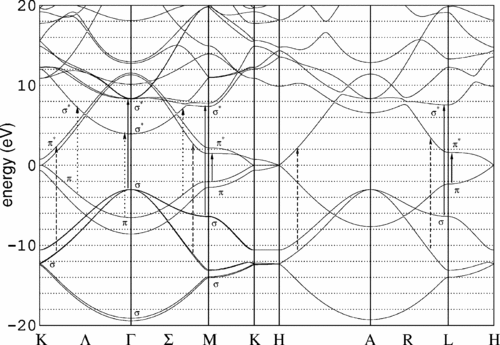
\includegraphics[width=.5\textwidth]{medium.png}
		\caption{Band structure of graphite, from Ref.~\cite{Graphite}.}
		\label{f7}
	\end{figure}

	Glass is an amorphous solid; that is, it does not have a crystal structure~\cite[pp.~573--674]{Kittel}.  Only solids with crystal structure have an energy band structure~\cite[p.~161]{Kittel}.  In order to absorb visible light, glass would need a band structure with the spacing between bands corresponding to optical frequencies.   Glass does not have this (or any) band structure, and a large gap between energy levels, so it cannot absorb visible light.  Moreover, glass is a nonmetal and so does not have free electrons, meaning it cannot appreciably reflect light.  Finally, since glass is created by cooling a liquid without crystallization~\cite[pp.~573--574]{Kittel}, it does not have structural impurities and thus does not scatter light.  Since glass does not appreciably absorb, reflect, or scatter visible light, it must only transmit it; this makes it transparent.
	
	Silver, in contrast, is a metal and therefore characterized by its abundance of free electrons in a partially filled energy band~\cite[p.~562]{Ashcroft}.  This means it has a high plasma frequency $\omgp^2 \propto n$ from (5.27), where $n$ is the free electron concentration.  We know from Fig.~\ref{f3d}~(left) that a Drude metal reflects light of all frequencies up to the plasma frequency; since $\omgp$ is large, it must be above the optical range.  This enables silver to reflect much of the optical light that is incident upon it.  In addition, the reflected waves interfere with light that would be transmitted.  So silver, like other metals, appears shiny because it almost exclusively reflects light.
	
	The band structure of graphite is shown in Fig.~\ref{f7}, which is from Ref.~\cite{Graphite}.  The de Broglie energy of visible light ranges from approximately 1.6 to \SI{3.3}{\electronvolt}~\cite[p.~1051]{YF}.  As the figure illustrates, graphite has many energy bands, and the spacing between them allows for band-to-band transmissions at nearly all optical frequencies.  This means that nearly all visible light that is incident upon graphite is absorbed, creating its black appearance.
	
	Table sugar is very pure, crystalline sucrose.  Granulated sugar is made up of small, nearly-transparent sucrose crystals with smooth edges~\cite{Sucrose}.  Powdered sugar is the result of grinding these crystals into a fine powder.  Since the grinding process results in many structural imperfections and harsh edges on the surface of the powdered sugar particles, they scatter visible light.  This gives powdered sugar its white appearance.
}